\documentclass[12pt]{article}
%\usepackage{psfig}
\usepackage{graphicx}
\usepackage{../lp}
\usepackage{amsmath}
% Cross-references for handout numbers.
\usepackage{amsfonts}
%\usepackage{amsthm}
\usepackage{hyperref}
\usepackage{amssymb}
%\usepackage[capitalize]{cleveref}
\usepackage{xcolor}

%\input{handouts}

\newcounter{chapnum}

\newtheorem{definition}{Definition}[chapnum]
\newtheorem{remark}{Remark}[chapnum]
\newtheorem{theorem}{Theorem}[chapnum]
\newtheorem{lemma}[theorem]{Lemma}
\newtheorem{corollary}[theorem]{Corollary}
\newtheorem{proposition}[theorem]{Proposition}
\newtheorem{claim}[theorem]{Claim}
\newtheorem{observation}{Observation}[chapnum]

\renewcommand{\thesection}{\arabic{chapnum}.\arabic{section}}
\renewcommand{\thefigure}{\arabic{chapnum}.\arabic{figure}}


\newenvironment{proof}{\noindent{\bf Proof:} \hspace*{1em}}{
        \hspace*{\fill} $\triangle$ }
\newenvironment{proof_of}[1]{\noindent {\bf Proof of #1:}
        \hspace*{1em} }{\hspace*{\fill} $\triangle$ }
\newenvironment{proof_claim}{\begin{quotation} \noindent}{
        \hspace*{\fill} $\diamond$ \end{quotation}}
\newenvironment{solution}{\noindent{\bf Solution:} \hspace*{1em}}{
        \hspace*{\fill} $\triangle$ }


\newcommand{\R}{{\mathbb R}}
\newcommand{\Z}{{\mathbb Z}}
\newcommand{\Q}{{\mathbb Q}}
\newcommand{\C}{{\mathbb C}}
\newcommand{\N}{{\mathbb N}}
\newcommand{\lin}{\operatorname{lin}}
\newcommand{\aff}{\operatorname{aff}}
\newcommand{\cone}{\operatorname{cone}}
\newcommand{\conv}{\operatorname{conv}}
\newcommand{\vol}{\operatorname{vol}}
\newcommand{\poly}{\operatorname{poly}}




\newcommand{\CF}[1]{{\color{purple}[CF: #1]}}


\newlength{\toppush}
\setlength{\toppush}{2\headheight}
\addtolength{\toppush}{\headsep}

\newcommand{\htitle}[2]{\noindent\vspace*{-\toppush}\newline\parbox{6.5in}
{Massachusetts Institute of Technology \hfill 18.453: Combinatorial Optimization 
\newline
\textbf{Instructor:} Cole Franks \quad \textbf{Notes: }Michel Goemans and Zeb Brady \hfill#2\newline
\mbox{}\hrulefill\mbox{}}\vspace*{1ex}\mbox{}\newline
\begin{center}{\Large\bf #1}\end{center}}

\newcommand{\handout}[2]{\thispagestyle{empty}
 \markboth{ #1 \hfil #2}{ #1 \hfil #2}
 \pagestyle{myheadings}\htitle{#1}{#2}}


\setlength{\oddsidemargin}{0pt}
\setlength{\evensidemargin}{0pt}
\setlength{\textwidth}{6.5in}
\setlength{\topmargin}{0in}
\setlength{\textheight}{8.5in}


\newcounter{exercisenum}
\newcounter{exercisetot}
\setcounter{exercisetot}{0}



\newenvironment{exercises}{
	\begin{list}{{\bf Exercise \arabic{chapnum}-\arabic{exercisenum}. \hspace*{0.5em}}}
	{\setlength{\leftmargin}{0em}
	 \setlength{\rightmargin}{0em}
	 \setlength{\labelwidth}{0em}
	 \setlength{\labelsep}{0em}
	\usecounter{exercisenum}
      \setcounter{exercisenum}{\theexercisetot}}}{\setcounter{exercisetot}{\theexercisenum}\end{list}}


\newenvironment{pseudocode}{
    \begin{list}{}{
        \renewcommand{\makelabel}{$\triangleright$}
        \setlength{\topsep}{0pt}
        \setlength{\leftmargin}{32pt}
        \setlength{\labelwidth}{14pt}
        \setlength{\labelsep}{0mm}
        \setlength{\itemindent}{0mm}
        \setlength{\itemsep}{-3pt}
        \setlength{\itemsep}{0mm}
        \setlength{\parsep}{0pt}%
        \setlength{\listparindent}{0pt}
    }
}
{
    \end{list}
}


\setcounter{chapnum}{6}
\newcommand{\F}{{\mathbb F}}
\newcommand{\spn}{\operatorname{span}}


\begin{document}
\handout{\arabic{chapnum}. Lecture notes on matroid
intersection}{\today}

One nice feature about matroids is that a simple greedy algorithm
allows to optimize over its independent sets or over its bases. At the
same time, this shows the limitation of the use of matroids: for many
combinatorial optimization problems, the greedy algorithm does not
provide an optimum solution. Yet, as we will show in this chapter, the
expressive power of matroids become much greater once we consider the
{\it intersection} of the family of independent sets of {\it two}
matroids. 

Consider two matroids $M_1=(E, {\cal I}_1)$ and $M_2=(E, {\cal I}_2)$
on the same ground set $E$, and consider the family of indepedent sets
common to both matroids, ${\cal I}_1 \cap {\cal I}_2$. This is what is
commonly referred to as the intersection of two matroids. 

In this chapter, after giving some examples of matroid intersection,
we show that that finding a largest common independent set to 2
matroids can be done efficiently, and provide a min-max relation for
the maximum value. We also consider the weighted setting (generalizing
the assignment problem), although we will not give an algorithm in the
general case (although one exists); we only restrict to a special
case, namely the arborescence problem. We shall hint an algorithm for
the general case by characterizing the matroid intersection polytope
and thereby giving a min-max relation for it (an NP$\cap$co-NP
characterization). Finally, we discuss also {\it matroid union}; a
powerful way to construct matroids from other matroids in which
matroid intersection plays a central role. (The term 'matroid union'
is misleading as it is not what we could expect after having defined
matroid intersection... it does {\it not} correspond to ${\cal I}_1\cup
{\cal I}_2$.)

\section{Examples}
\subsection{Bipartite matchings}
Matchings in a bipartite graph $G=(V,E)$ with bipartition $(A,B)$ do
not form the independent sets of a matroid. However, they can be
viewed as the common independent sets to two matroids; this is the
canonical example of matroid intersection. 

Let $M_A$  be a partition matroid with ground set $E$ where the
partition of $E$ is given by $E=\bigcup\{\delta(v): v\in A\}$ where
$\delta(v)$ denotes the edges incident to $v$. Notice that this is a
partition since all edges have precisely one endpoint in $A$. We also
define $k_v=1$ for every $v\in A$. Thus, the family of independent
sets of $M_A$ is given by 
$${\cal I}_A=\{F: |F\cap\delta(v)|\leq 1 \mbox{ for all } v\in A\}.$$
In other words, a set of edges is independent for $M_A$ if it has
at most one edge incident to every vertex of $A$ (and any number of
edges incident to every vertex of $b$). 
 We can similarly define $M_B=(E,{\cal I}_B)$ by
$${\cal I}_B=\{F: |F\cap\delta(v)|\leq 1 \mbox{ for all } v\in B\}.$$
Now observe that any $F\in {\cal I}_A\cap {\cal I}_B$ corresponds to a
matching in $G$, and vice versa. And the largest common independent
set to ${\cal I}_A$ and ${\cal I}_B$ corresponds to a maximum matching
in $G$. 

\subsection{Arborescences}
Given a digraph $D=(V,A)$ and a special root vertex $r\in V$, an
$r$-arborescence (or just arborescence) is a spanning tree (when
viewed as an undirected graph) directed
away from $r$. Thus, in a $r$-arborescence, every vertex is reachable
from the root $r$. As an $r$-arborescence has no arc incoming to the
root, we assume that $D$ has no such arc.

$r$-arborescences can be viewed as sets simultaneously independent in
two matroids.  Let $G$ denote the undirected counterpart of $D$
obtained by disregarding the directions of the arcs. If
have both arcs $a_1=(u,v)$ and $a_2=(v,u)$ in $D$, we define $G$ to have two
undirected edges also labelled $a_1$ and $a_2$ between $u$ and $v$ (i.e. $G$ might be a multigraph). Define $M_1=(A,{\cal I}_1)=M(G)$ the graphic matroid corresponding
to $G$, and $M_2=(A,{\cal I}_2)$ the partition matroid in which
independent sets are those with at most one arc incoming to every
vertex $v\neq r$. In other words, we let $${\cal I}_2=\{F: |F\cap
\delta^-(v)|\leq 1 \mbox{ for all } v\in V\setminus \{r\}\} $$ where
$\delta^-(v)$ denotes the set $\{(u,v)\in A\}$ of arcs incoming to
$v$. Thus, any $r$-arborescence is independent in both matroids $M_1$
and $M_2$. Conversely, any set $T$ independent in both $M_1$ and $M_2$
and of cardinality $|V|-1$ (so that it is a base in both matroids) is
an $r$-arborescence. Indeed, such a $T$ being a spanning tree in $G$
has a unique path between $r$ and any vertex $v$; this path must be
directed from the root $r$ since otherwise we would have either an arc
incoming to $r$ or two arcs incoming to the same vertex. 

In the minimum cost arborescence problem, we are also given a cost
function $c: A \rightarrow \R$ and we are interested in finding the
minimum cost $r$-arborescence. This is a directed counterpart to the
minimum spanning tree problem but, here, the greedy algorithm does not
solve the problem.   

\subsection{Orientations}

Given an undirected graph $G=(V,E)$, we consider orientations of all
its edges into directed arcs; namely, each (undirected)
edge\footnote{Usually, we use $(u,v)$ to denote an (undirected)
  edge. In this section, however, we use the notation $\{u,v\}$ rather
  than $(u,v)$ to emphasize that edges are undirected.} $\{u,v\}$
is either replaced by an arc\footnote{We use arcs in the case of
directed graphs, and edges for undirected graphs.}  $(u,v)$ from $u$
to $v$, or by an arc $(v,u)$ from $v$ to $u$. Our goal is, given $k: V
\rightarrow \N$, to decide whether there exists an orientation such
that, for every vertex $v\in V$, the indegree of vertex $v$ (the
number of arcs entering $v$) is at most $k(v)$. Clearly, this is not
always possible, and this problem can be solved using matroid
intersection (or network flows as well).

To attack this problem through matroid intersection, consider the
directed graph $D=(V,A)$ in which every edge $e=\{u,v\}$ of $E$ is
replaced by two arcs $(u,v)$ and $(v,u)$. With the arc set $A$ as
ground set, we define two partition matroids, $M_1$ and $M_2$. To be
independent in $M_1$, one can take at most one of $\{(u,v),(v,u)\}$
for every $(u,v)\in E$, i.e.
$${\cal I}_1=\{F\subseteq A: |F\cap \{(u,v),(v,u)\}|\leq 1 \mbox{ for
  all } (u,v)\in E\}.$$
To be independent in $M_2$, one can take at
most $k(v)$ arcs among $\delta^-(v)$ for every $v$:
$${\cal I}_2=\{F\subseteq A: |F\cap \delta^-(v)|\leq k(v) \mbox{ for
  all } v\in V\}.$$ Observe that this indeed defines a partition
  matroid since the sets $\delta^-(v)$ over all $v$ partition $A$. 

Therefore, there exists an orientation satisfying the required
indegree restrictions if there exists a common independent set to
$M_1$ and $M_2$ of cardinality precisely $|E|$ (in which case we select
either $(u,v)$ or $(v,u)$ but not both).  

\subsection{Colorful Spanning Trees}
Suppose we have an undirected graph $G=(V,E)$ and every edge has a
color. This is represented by a partition of $E$ into $E_1\cup \cdots
\cup E_k$ where each $E_i$ represents a set of edges of the same
color $i$. The problem of deciding whether this graph has a spanning tree
in which all edges have a different color can be tackled through
matroid intersection. Such a spanning tree is called {\it colorful}. 

Colorful spanning trees are bases of the graphic matroid $M_1=M(G)$ which
are also independent in the partition matroid $M_2=(E,{\cal I}_2)$
defined by ${\cal I}_2=\{F: |F\cap E_i|\leq 1 \mbox{ for all } i\}$. 

\subsection{Union of Two Forests}
In Section \ref{matroidunion}, we show that one can decide whether a graph
$G$ has two edge-disjoint spanning trees by matroid intersection. 


\section{Largest Common Independent Set}
As usual, one issue is to find a common independent set of largest
cardinality, another is to prove that indeed it is optimal. This is
done through a min-max relation. 

Given two matroids $M_1=(E, {\cal I}_1)$ and $M_2=(E, {\cal I}_2)$
with rank functions $r_1$ and $r_2$ respectively, consider any set
$S\in {\cal I}_1\cap {\cal I}_2$ and any $U\subseteq E$. Observe that
$$|S|=|S\cap U|+ |S\cap (E\setminus U)| \leq r_1(U) + r_2(E\setminus
U),$$ since both $S\cap U$ and $S\cap (E\setminus U)$ are independent
in $M_1$ and in $M_2$ (by property $(I_1)$); in particular (and this
seems weaker), $S\cap U$ is independent for $M_1$ while $S\cap
(E\setminus U)$ is independent for $M_2$. Now, we can take the maximum
over $S$ and the minimum over $U$ and derive:
$$\max_{S\in {\cal I}_1 \cap {\cal I}_2} |S| \leq \min_{U\subseteq E}
\left[ r_1(U) + r_2(E\setminus U)\right].$$
Somewhat surprisingly, we will show that we always have equality:
\begin{theorem}[Matroid Intersection] \label{thm:matint}
For any two matroids  $M_1=(E, {\cal I}_1)$ and $M_2=(E, {\cal I}_2)$
with rank functions $r_1$ and $r_2$ respectively, we have:
\begin{equation} \label{eqminmax}
\max_{S\in {\cal I}_1 \cap {\cal I}_2} |S| =\min_{U\subseteq E}
\left[ r_1(U) + r_2(E\setminus U)\right].
\end{equation}
\end{theorem}

Before describing an algorithm for matroid intersection that proves
this theorem, we consider what the min-max result says for some special
cases. First, observe that we can always restrict our attention to
sets $U$ which are closed for matroid $M_1$. Indeed, if that was not
the case, we could replace $U$ by $V=\operatorname{span}_{M_1}(U)$ and we would have
that $r_1(V)=r_1(U)$ while $r_2(E\setminus V)\leq r_2(E\setminus
U)$. This shows that there always exists a set $U$ attaining the
minimum which is closed for $M_1$. Similarly, we could assume that
$E\setminus U$ is closed for $M_2$ (but both assumptions cannot be
made simultaneously).  

% For the $r$-arborescence problem, 

When specializing the matroid intersection theorem to  the
graph orientation problem discussed earlier in this chapter, we can
derive the following. 
\begin{theorem}
$G=(V,E)$ has an orientation such that the indegree of vertex $v$ is
at most $k(v)$ for every $v\in V$ if and only if for all $P\subseteq
V$ we have\footnote{$E(P)$ denotes the set of edges with both endoints
  in $P$.}:
$$|E(P)|\leq \sum_{v\in P} k(v).$$
\end{theorem}

Similarly, for colorful spanning trees, we obtain:
\begin{theorem}
Given a graph $G=(V,E)$ with edges of $E_i$ colored $i$ for
$i=1,\cdots, k$, there exists a colorful spanning tree if and only if
deleting the edges of any $c$ colors (for any $c\in \N$) produces at
most $c+1$ connected components. 
\end{theorem}

We now prove Theorem \ref{thm:matint} by exhibiting  an algorithm
for finding a maximum cardinality independent set common to two
matroids and a corresponding set $U$ for which we have equality in
(\ref{eqminmax}).  For
the algorithm, we will start with $S = \emptyset$ and at each step
either augment $S$ or produce a $U$ that gives equality. Our algorithm
will rely heavily on a structure called the exchange graph. We first
focus on just one matroid. 

\begin{definition} Given a matroid $M = (E,\mathcal{I})$ and an
independent set $S \in \mathcal{I}$, the \emph{exchange graph}
$\mathcal{G}_M(S)$ (or just $\mathcal{G}(S)$) is the bipartite graph
with bipartition $S$ and $E \setminus S$ with an edge between $y \in
S$ and $x \in E\setminus S$ if $S-y+x \in \mathcal{I}$.
\end{definition}

\begin{lemma} \label{lem:match} Let $S$ and $T$ be two independent
sets in $M$ with $|S| = |T|$. Then there exists a perfect matching
between $S \setminus T$ and $T \setminus S$ in $\mathcal{G}_M(S)$.
\end{lemma}

%\begin{proof} 
%\end{proof}


The proof is omitted. The converse to Lemma \ref{lem:match} does not
hold. We next prove a proposition that is a partial converse to the
above lemma. The next proposition can also be thought of as a generalization of the fact that an upper triangular matrix with $1$s on the diagonal has full rank.

\begin{proposition} Let $S \in \mathcal{I}$ with exchange graph
$\mathcal{G}_M(S)$. Let $T$ be a set with $|T| = |S|$ and such that
$\mathcal{G}_M(S)$ has a \emph{unique} perfect matching between $S \setminus
T$ and $T \setminus S$. Then $T \in \mathcal{I}$.  \end{proposition}

\begin{proof} Let $N$ be the unique matching. We claim that we can choose orderings $S \setminus T = (y_1, \dots, y_t)$ and $T \setminus S = (x_1, \dots, x_t)$ such that $N =
\{(y_1,x_1),(y_2,x_2),\ldots,(y_t,x_t)\}$ and that $(y_i,x_j)$ is
never an edge of $G_M(S)$ for $i < j$.

To prove this, orient edges in $N$ from
$T \setminus S$ to $S\setminus T$, and orient the rest of the edges between $S \setminus T$ and $T \setminus S$ in $G_M(S)$ from
$S\setminus T$ to $T \setminus S$. We'll ignore all edges in $G_M(S)$ not between $S \setminus T$ and $T \setminus S$. If we contract the edges of the matching $N$,
observe that the resulting directed graph with $|S\setminus T| =|T\setminus S| = t$ vertices has no directed cycle since,
otherwise, we could find an alternating cycle prior to contraction,
and this would contradict the uniqueness of the matching. Thus we may order the vertices of the contracted graph as $z_1, \dots, z_t$ (using a topological ordering) such that there are no directed edges $(z_i, z_j)$ for $j > i$. Letting $y_i, x_i$ be the vertices of $S\setminus T$ and $T\setminus S$, respectively, contracted to form $z_i$ results in the desired orderings.

Now suppose for the sake of contradiction that $T \not\in
\mathcal{I}$. Then $T$ contains a circuit $C$. Take the smallest $i$ such
that $x_i \in C$ (there must exist at least one element of $C$ in $T
\setminus S$ since $C \subseteq T$ and $S$ is independent). By
construction, $(y_i,x)$ is not an edge for $x \in C-x_i$. This implies
that $x \in \spn(S-y_i)$ for all $x \in C-x_i$. Hence $C-x_i \subseteq
\spn(S-y_i)$, so $\spn(C-x_i) \subseteq \spn(\spn(S-y_i)) =
\spn(S-y_i)$. $C$ is a circuit, so $x_i \in \spn(C-x_i)$, and thus $x_i \in
\spn(S-y_i)$. This is a contradiction, since $(y_i,x_i) \in
\mathcal{G}_M(S)$ by assumption. Therefore $T$ must be in
$\mathcal{I}$, which proves the proposition.  \end{proof}

We are now ready to describe the algorithm for proving the minmax
formula. First, we define a new type of exchange graph for the case
when we are dealing with two matroids. 

\begin{definition} For $S \in \mathcal{I}_1 \cap \mathcal{I}_2$, the
exchange graph $\mathcal{D}_{M_1,M_2}(S)$ is the directed bipartite
graph with bipartition $S$ and $E \setminus S$ such that $(y,x)$ is
an arc if $S-y+x \in \mathcal{I}_1$ and $(x,y)$ is an arc if $S-y+x
\in \mathcal{I}_2$.  \end{definition}

Also define $X_1 := \{x \not\in S \mid S+x \in \mathcal{I}_1\}$, the
set of {\it sources}, and
$X_2 := \{x \not\in S \mid S+x \in \mathcal{I}_2\}$, the set of {\it sinks}. Then the
algorithm is to find a path (we call it an \emph{augmenting path})
from $X_1$ to $X_2$ that does not contain any shortcuts (arcs that
point from an earlier vertex on the path to a non-adjacent later
vertex on the path). This for example can be obtained by selecting a
shortest path from $X_1$ to $X_2$. Then replace $S$ with $S \triangle P$, where $P$
is the set of vertices on the path. As a special case, if $X_1 \cap
X_2 \neq \emptyset$, then we end up with a path that consists of a
singleton vertex and we can just add that element to $S$.  If there is
no such path, then set $U := \{z \in E \mid z \text{ can reach some
vertex in } X_2 \text{ in }
\mathcal{D}_{M_1,M_2}(S)\}$. Alternatively, we could define
$E\setminus U$ as the set of vertices which can be reached from a
vertex in $X_1$; this may give a different set. 

To prove that this algorithm is correct, we need to show that
\begin{enumerate} \item When we stop, the sets $S$ and $U$ do indeed
give equality in the minmax formula (\ref{eqminmax}).

\item At each stage in the algorithm, $S \triangle P \in \mathcal{I}_1
\cap \mathcal{I}_2$.  \end{enumerate}

\begin{proof_of}{1} First note that $X_2 \subseteq U$ and that $X_1
\cap U = \emptyset$ (as otherwise we could keep running the algorithm
to increase the size of $S$). We claim that $r_1(U) = |S \cap U|$ and
$r_2(E \setminus U) = |S \cap (E \setminus U)|$. Together, these
would imply that $|S| = r_1(U)+r_2(E \setminus U)$, which is what we
need.

Suppose first that $|S \cap U| \neq r_1(U)$. Since $S \cap U \subseteq
U$ and $S \cap U$ is independent, this would imply that $|S \cap U| <
r_1(U)$. Then there would have to exist some $x \in U \setminus S$
such that $(S \cap U)+x \in \mathcal{I}_1$. As $S\in \mathcal{I}_1$,
we can repeatedly add elements of $S$ to $(S \cap U)+x$ and thereby
obtain a set of the form $S+x-y$ for some $y \in S \setminus U$ with
$S+x-y\in \mathcal{I}_1$. But then $(y,x)$ is an arc in
$\mathcal{D}_{M_1,M_2}(S)$, so $y \in U$ (since $x \in U$). This is a
contradiction, so we must have $|S \cap U| = r_1(U)$.

Now suppose that $|S \cap (E \setminus U)| \neq r_2(E \setminus
U)$. Then as before we must have $|S \cap (E \setminus U)| < r_2(S
\setminus U)$. Thus there exists $x \in (E \setminus U) \setminus
S$ such that $(S \cap (E \setminus U)) + x \in \mathcal{I}_2$. So, by
the same logic as before, we can find $y \in S \setminus (E
\setminus U)$ such that $S-y+x \in \mathcal{I}_2$. But $S \setminus
(E \setminus U) = S \cap U$, so we have $y \in S \cap U$ such that
$S-y+x \in \mathcal{I}_2$. But then $(x,y)$ is an arc in
$\mathcal{D}_{M_1,M_2}(S)$, so $x \in U$ (since $y \in U$). This is a
contradiction, so we must have $|S \cap (E \setminus U)| = r_2(E
\setminus U)$.  \end{proof_of}


%%% different proof than in the lecture notes

\begin{proof_of}{2} Recall that we need to show that $S \triangle P
\in \mathcal{I}_1 \cap \mathcal{I}_2$ whenever $P$ is a path from
$X_1$ to $X_2$ with no shortcuts. We first show that $S \triangle P
\in \mathcal{I}_1$. We start by defining a new matroid $M_1'$ from
$M_1$. To do so, add a new element $t$ to $E$ (thought of as a sink) and define $M_1' := (E \cup \{t\},\{J \mid J \setminus \{t\} \in
\mathcal{I}_1\}$. In other words, we simply add a new element $\{t\}$
that is independent from all the other elements of the matroid. Then
we know that $S \cup \{t\}$ is independent in $M_1'$ and $M_2'$ (where
we define $M_2'$ analogously to $M_1'$). On the other hand, if we view
$G_{M_1'}(S \cup \{t\})$ as a subgraph of
$G_{M_1',M_2'}(S \cup \{t\})$, then there exists a perfect
matching in $\mathcal{G}_{M_1'}(S \cup \{t\})$ between $(S \cap P)
\cup \{t\}$ and $P \setminus S$ (given by the arcs in $P$ that are
also arcs in $\mathcal{D}_{M_1'}(S \cup \{t\})$, together with the arc
between $\{t\}$ and the first vertex in $P$). Furthermore, this
matching is unique since $P$ has no shortcuts, so by the proposition
we know that $(S \cup \{t\}) \triangle P$ is independent in $M_1'$,
hence $S \triangle P$ is independent in $M_1$.

The proof that $S \triangle P \in \mathcal{I}_2$ is identical, except
that this time the matching consists of the arcs in $P$ that are also
arcs in $\mathcal{D}_{M_2'}(S \cup \{t\})$, together with the arc
between $\{t\}$ and the \emph{last} vertex in $P$ (rather than the
first).  \end{proof_of}

So, we have proved that our algorithm is correct, and as a consequence
have established the minmax formula.




\begin{exercises}
\item
Deduce K\"onig's theorem about the maximum size of a matching in a
bipartite graph from the min-max relation for the maximum independent
set common to two matroids. 
\end{exercises}

\section{Matroid Intersection Polytope}

In this section, we characterize the {\it matroid intersection
polytope} in terms of linear inequalities,
that is the convex hull of characteristic vectors of independent sets
common to two matroids. Let $M_1=(E,\mathcal{I}_1)$ and
$M_2=(E,\mathcal{I}_2)$ be two matroids, and let
$$X=\{\chi(S)\in\{0,1\}^{|E|}: S\in \mathcal{I}_1\cap
\mathcal{I}_2\}.$$ The main result is that $conv(X)$ is precisely given by the
intersection of the matroid polytopes for $M_1$ and $M_2$.  

\begin{theorem} \label{matintpol}
Let $$\begin{array}{rll} 
P = \{x\in \R^{|E|}: & x(S) \leq r_1(S) & \forall S\subseteq E \\
& x(S) \leq r_2(S) & \forall S\subseteq E \\
& x_e \geq 0 & \forall e\in E\}
\end{array}.$$
Then $conv(X)=P$. 
\end{theorem}

Our proof will be vertex-based. We will show that any extreme point of
$P$ is integral, and it can then be easily seen that it corresponds to
a common independent set. The proof will rely on total unimodularity
in a subtle way. Even though the overall matrix defining $P$ is {\it
not} totally unimodular, we will show that, for every extreme point
$x^*$, $x^*$ can be seen as the solution of a system of equations
whose underlying matrix is totally unimodular. This is a powerful
approach that can apply to many settings.  

\begin{proof}
Let $x^*$ be an extreme point of $P$. We know that $x^*$ is uniquely
characterized once we know the inequalities that are tight in the
description of $P$. Let $$\mathcal{F}_i=\{S\subseteq E:
x^*(S)=r_i(S)\},$$ for $i=1,2$. Let $E_0=\{e\in E: x^*_e=0\}$. We know
that $x^*$ is the unique solution to 
$$\begin{array}{ll}
x(S)=r_1(S) & S\in \mathcal{F}_1 \\
x(S)=r_2(S) & S \in \mathcal{F}_2 \\
x_e = 0 & e\in E_0.
\end{array}$$
Consider the matroid polytope $P_i$ for matroid $M_i$ for $i=1,2$, and
define the face $F_i$ of $P_i$ (for $i=1,2$) to be 
$$\begin{array}{rll} 
F_i = \{x\in P_i: & x(S) = r_i(S) & \forall S\in \mathcal{F}_i\\
& x_e =0 & \forall e\in E_0\}
\end{array}.$$
Observe that $F_1\cap F_2=\{x^*\}$. Also, by Theorem 5.6 of the
chapter on matroid optimization, we have that $F_i$ can be
alternatively defined by a {\it chain} $\mathcal{C}_i$. Thus, $x^*$ is
the unique solution to
$$\begin{array}{ll}
x(S) = r_1(S) & S\in \mathcal{C}_1 \\
x(S) = r_2(S) & S\in \mathcal{C}_2 \\
x_e=0 & e\in E_0.
\end{array}$$
After eliminating all variables in $E_0$, this system can be written
as $Ax=b$, where the rows of $A$ are the characteristic vectors of
$\mathcal{C}_1 \cup \mathcal{C}_2$. 

Such a matrix $A$ is totally unimodular and this can be shown by using
Theorem 3.14. Consider any subset of rows; this corresponds to
restricting our attention to chains $\mathcal{C}'_1$ and
$\mathcal{C}'_2$. Consider first $\mathcal{C}'_1$. If we assign the largest set to $R_1$ and then keep
alternating the assignment between $R_2$ and $R_1$ as we consider
smaller and smaller sets, we obtain that 
$$\sum_{i\in \mathcal{C}'_1\cap R_1} a_{ij} - \sum_{i\in
\mathcal{C}'_1\cap R_2} a_{ij}\in \{0,1\},$$ for all $j$. If for
$\mathcal{C}'_2$ we start with the largest set being in  $R_2$, we get
$$\sum_{i\in \mathcal{C}'_2\cap R_1} a_{ij} - \sum_{i\in
\mathcal{C}'_2\cap R_2} a_{ij}\in \{0,-1\},$$ for all $j$. Combining
both, we get that indeed for every $j$, we get a value in $\{0,1,-1\}$
showing that the matrix is totally unimodular. As a result, $x^*$ is
integral, and therefore corresponds to the characteristic vector of a
common independent set. 
\end{proof}

\section{Arborescence Problem}


The minimum cost $r$-arborescence is the problem of, given a directed
graph $D=(V,A)$, a root vertex $r\in V$ and a cost $c_a$ for every arc
$a\in A$, finding an $r$-arborescence in $D$ of minimum total cost. This
can thus be viewed as a weighted matroid intersection problem and we
could use the full machinery of matroid intersection algorithms and
results. However, here, we are going  to develop a simpler  algorithm
using notions similar to the Hungarian method for the assignment
problem. We will assume that the costs are nonnegative. 

As an integer program, the problem can be formulated as
follows. Letting $x_a$ be 1 for the arcs of an $r$-arborescence, we
have the formulation: 

\lps 
& OPT & = & \min &\sum_{a\in A} c_a x_a \\
\\ & \lefteqn{\mbox{subject to:}} \\
& & & & \sum_{a\in \delta^-(S)} x_a \geq 1 & \forall S\subseteq
V\setminus\{r\} \\
& &  & &\sum_{a\in \delta^-(v)} x_a = 1 & \forall v\in V\setminus\{r\} \\
& & & & x_a \in \{0,1\} & a\in A.
\elps

In this formulation $\delta^-(S)$ represents the set of arcs
$\{(u,v)\in A: u\notin S, v\in S\}$. One can check that any feasible
solution to the above corresponds to the incidence vector of an
$r$-arborescence.  Notice that this optimization problem has an
exponential number of constraints. We are going to show that we can
relax both the integrality restrictions to $x_a\geq 0$ and also remove
the equality constraints $\sum_{a\in \delta^-(v)} x_a = 1$ and still
there will be an $r$-arboresence that will be optimum for this relaxed
(now linear) program. The relaxed linear program (still with an
exponential number of constraints) is:

\lps 
& LP & = & \min & \sum_{a\in A} c_a x_a \\
\\ & \lefteqn{\mbox{subject to:}} \\
(P) & & & & \sum_{a\in \delta^-(S)} x_a \geq 1 & \forall S\subseteq
V\setminus\{r\} \\
& & & & x_a \geq 0 & a\in A.
\elps

The dual of this linear program is:
\lps
& LP & = & \max & \sum_{S\subseteq
V\setminus\{r\} } y_S \\
\\ & \lefteqn{\mbox{subject to:}} \\
(D) & & & & \sum_{S: a\in \delta^-(S)} y_S \leq c_a \\
& & & & y_S \geq 0 & S\subseteq
V\setminus\{r\}.
\elps

The algorithm will be constructing an arborescence $T$ (and the
corresponding incidence vector $x$ with $x_a=1$ whenever $a\in T$ and
0 otherwise) and a feasible
dual solution $y$ which satisfy complementary slackness, and this will
show that $T$ corresponds to an optimum solution of $(P)$, and hence is
an optimum arborescence. Complementary slackness says:
\begin{enumerate}
\item
$y_S>0 \Longrightarrow | T \cap \delta^-(S)| =1$, and
\item
$a\in T \Longrightarrow \sum_{S: a\in \delta^-(S)} y_S = c_a$.
\end{enumerate}
The algorithm will proceed in 2 phases. In the first phase, it will
construct a dual feasible solution $y$ and a set $F$ of arcs which has
a directed path from the root to every vertex. This may not be an
$r$-arborescence as there might be too many arcs. The arcs in $F$ will
satisfy condition 2 above (but not condition 1). In the second phase,
the algorithm will remove unnecessary arcs, and will get an
$r$-arborescence satisfying condition 1.

Phase 1 is initialized with $F=\emptyset$ and $y_S=0$ for all
$S$, and a counter $k=1$. While $F$ does not contain a directed path to every vertex in
$V$, the algorithm selects a set $S$ such that (i) inside $S$, $F$ is
strongly connected (i.e. every vertex can reach every vertex) and (ii)
$F\cap \delta^-(S)=\emptyset$. This set $S$ exists since we can
contract all strongly connected components and in the resulting
acyclic digraph, there must be a vertex (which may be coming from the
shrinking of a strongly connected component) with no incoming arc
(otherwise tracing back from that vertex we would either get to the
root or discover a new directed cycle (which we could shrink)). Now we
increase $y_S$ as much as possible until a new inequality, say for arc
$a_k$, $\sum_{S: a_k\in \delta^-(S)} y_S \leq c_{a_k}$ becomes an
equality. In so doing, the solution $y$ remains dual feasible and
still satisfies condition 2. We can now add $a_k$ to $F$ without
violating complementary slackness condition 2, and then we increment
$k$ (which at the start we initialized at $k=1$). And we continue by
selecting another set $S$, and so on, until every vertex is reachable
from $r$ in $F$. We have now such a set $F=\{a_1,a_2,\cdots,a_k\}$ and
a dual feasible solution $y$ satisfying condition 2.

In step 2, we eliminate as many arcs as possible, but we consider them
in {\it reverse order} they were added to $F$. Thus, we let $i$ go
from $k$ to 1, and if $F\setminus\{a_i\}$ still contains a directed
path from $r$ to every vertex, we remove $a_i$ from $F$, and
continue. We then output the resulting set $T$ of arcs.

The first claim is that $T$ is an arborescence. Indeed, we claim it has
exactly $|V|-1$ arcs with precisely one arc incoming to every vertex
$v\in V\setminus\{r\}$. Indeed, if not, there would be two arcs $a_i$
and $a_j$ incoming to some vertex $v$; say that $i<j$. In the reverse
delete step, we should have removed  $a_j$; indeed any vertex
reachable from $r$ through $a_j$ could be reached through $a_i$ as
well (unless $a_i$ is unnecessary in which case we could get rid of
$a_i$ later on).

The second (and final) claim is that the complementary slackness
condition 1 is also satisfied. Indeed, assume not, and assume that we
have a set $S$ with $y_S>0$ and $|T \cap \delta^-(S)|>1$. $S$ was
chosen at some point by the algorithm and at that time we added
$a_k\in \delta^-(S)$ to $F$. As there were no other arcs in
$\delta^-(S)$ prior to adding $a_k$ to $F$, it means that all other arcs
in $T\cap \delta^-(S)$ must be of the form $a_j$ with $j>k$. In
addition, when $S$ was chosen, $F$ was already strongly connected
within $S$; this means that from any vertex inside $S$, one can go  to
any other vertex inside $S$ using arcs $a_i$ with $i<k$. We claim that
when $a_j$ was considered for removal, it should have been
removed. Indeed, assume that $a_j$ is needed to go to vertex $v$, and
that along the path $P$ to $v$ the last vertex in $S$ is $w\in S$. Then we
could go to $v$ by using $a_k$ which leads somewhere in $S$ then take
arcs $a_i$ with $i<k$ (none of which have been removed yet as $i<k<j$)
to $w\in S$ and then continue along path $P$. So $a_j$ was not really
necessary and should have been removed. This shows that complementary
slackness condition 1 is also satisfied and hence the arborescence
built is optimal. 

\section{Matroid Union} \label{matroidunion}

From any matroid $M=(E,{\cal I})$, one can construct a dual matroid
$M^*=(E, {\cal I}^*)$.  

\begin{theorem} \label{dual}
Let ${\cal I}^*=\{X \subseteq E: E\setminus X$ contains a
base of $M\}$. Then $M^*=(E,{\cal I}^*)$ is a matroid with rank
function
$$ r_{M^*}(X)=|X|+r_M(E\setminus X)-r_M(E).$$
\end{theorem}

There are several ways to show this. One is to first show that indeed
the size of the largest subset of $X$ in ${\cal I}^*$  has
cardinality $|X|+r_M(E\setminus X)-r_M(E)$ and then show that
$r_{M^*}$ satisfies the three  conditions that a rank function of a
matroid needs to satisfy (the third one, submodularity, follows
from the submodularity of the rank function for $M$). 

One can use Theorem \ref{dual} and matroid intersection to get a good
characterization of when a graph $G=(V,E)$ has two edge-disjoint spanning
trees. Indeed, letting $M$ be the graphic matroid of the graph $G$, we
get that $G$ has two edge-disjoint spanning trees if and only if 
$$\max_{S\in {\cal I} \cap {\cal I}^*} |S| = |V|-1.$$ For the
graphic matroid, we know that $r_M(F)=n -\kappa(F)$ where $n=|V|$ and
$\kappa(F)$ denotes the number of connected components of $(V,F)$.
But by the matroid intersection theorem, we can write:
\begin{eqnarray*}
\max_{S\in {\cal I}\cap {\cal I}^*} |S| & = &
\min_{E_1\subseteq E}\left[ r_M(E_1) + r_{M^*}(E\setminus E_1)\right] \\
 & = & \min_{E_1\subseteq E} \left[(n- \kappa(E_1)) + \left( |E\setminus E_1| +
\kappa(E)-\kappa(E_1)\right) \right] \\
& = &  \min_{E_1\subseteq E} \left[n + 1 + |E\setminus E_1| - 2
  \kappa(E_1) \right],
\end{eqnarray*}
where we replaced $\kappa(E)$ by 1 since otherwise $G$ wouldn't even have
one spanning tree. 
Rearranging terms, we get that $G$ has two edge-disjoint spanning trees
if and only if for all $E_1\subseteq E$, we have that $E\setminus E_1
\geq 2(\kappa(E_1)-1)$. If this inequality is violated for some $E_1$,
we can add to $E_1$ any edge that does not decrease $\kappa(E_1)$. In
other words, if the connected components of $E_1$ are $V_1$, $V_2,
\cdots, V_p$ then we can assume that $E_1=E\setminus \delta(V_1, V_2,
\cdots V_p)$ where $\delta(V_1, \cdots, V_p)=\{(u,v)\in E: u\in V_i,
v\in V_j $ and $i\neq j\}$. Thus we have shown:

\begin{theorem} \label{2edge}
$G$ has two edge-disjoint spanning trees if and only if for all
  partitions $V_1$, $V_2, \cdots V_p$ of $V$, we have 
$$ |\delta(V_1, \cdots, V_p)|\geq 2(p-1).$$
\end{theorem}

Theorem \ref{2edge} can be generalized to an arbitrary number of
edge-disjoint spanning trees. This result is not proved here. 

\begin{theorem} \label{kedge}
$G$ has $k$ edge-disjoint spanning trees if and only if for all
  partitions $V_1$, $V_2, \cdots V_p$ of $V$, we have 
$$ |\delta(V_1, \cdots, V_p)|\geq k(p-1).$$
\end{theorem}

From two matroids $M_1=(E, {\cal I}_1)$ and $M_2=(E, {\cal
I}_2)$, we can also define its union by $M_1\cup M_2=(E,{\cal I})$
where ${\cal I}=\{S_1\cup S_2: S_1\in {\cal I}_1, S_2\in {\cal
  I}_2\}$. Notice that we do not impose the two matroids to be
identical as we just did for edge-disjoint spanning trees. 

We can show that:
\begin{theorem}[Matroid Union] \label{thm:unionmatroid}
$M_1\cup M_2$ is a matroid. Furthermore its rank function is given by 
$$r_{M_1\cup M_2}(S)=\min_{F \subseteq S} \left\{ |S \setminus F| +
  r_{M_1}(F) + r_{M_2} (F) \right\}.$$
\end{theorem}

\begin{proof}
  To show that it is a matroid, assume that $X, Y \in {\cal I}$ with
  $|X|<|Y|$. Let $X=X_1\cup X_2$ and $Y=Y_1\cup Y_2$ where $X_1,
  Y_1\in {\cal I}_1$ and $X_2, Y_2\in {\cal I}_2$. We can furthermore
  assume that the $X_i$'s are disjoint and so are the $Y_i$'s. Finally
  we assume that among all choices for $X_1, X_2, Y_1$ and $Y_2$, we
  choose the one maximizing $|X_1\cap Y_1|+|X_2\cap Y_2|$. Since
  $|Y|>|X|$, we can assume that $|Y_1|>|X_1|$. Thus, there exists
  $e\in (Y_1\setminus X_1)$ such that $X_1\cup \{e\}$ is independent
  for $M_1$. The maximality implies that $e\notin X_2$ (otherwise
  consider $X_1\cup \{e\}$ and $X_2\setminus\{e\}$). But this implies
  that $X\cup \{e\}\in {\cal I}$ as desired.

We now show the expression for the rank function. The fact that it is
$\leq$ is obvious as an independent set $S\in {\cal I}$ has size
$|S\setminus F|+ |S\cap F|\leq |S\setminus F| + r_{M_1}(F)+r_{M_2}(F)$
and this is true for any $F$.

For the converse, let us prove it for the entire ground set
$S=E$. Once we  prove that 
 $$r_{M_1\cup M_2}(E)=\min_{F \subseteq S} \left\{ |E \setminus F| +
  r_{M_1}(F) + r_{M_2} (F) \right\},$$
the corresponding statement for any set $S$ will follow by just
restricting our matroids to $S$.
 
Let $X$ be a base of $M_1\cup M_2$. The fact that $X\in {\cal I}$
means that $X=X_1\cup X_2$ with $X_1\in {\cal I}_1$ and $X_2\in {\cal
  I}_2$. We can furthermore assume that $X_1$ and $X_2$ are disjoint
and that $r_{M_2}(X_2)=r_{M_2}(E)$ (otherwise add elements to $X_2$
and possibly remove them from $X_1$). Thus we can assume that
$|X|=|X_1|+ r_{M_2}(E)$. We have that $X_1\in {\cal I}_1$ and also
that $X_1$ is independent for the dual of $M_2$ (as the complement of
$X_1$ contains a base of $M_2$). In other words, $X_1\in {\cal I}_1
\cap {\cal I}^*_2$. The proof is completed by using the matroid
intersection theorem and Theorem \ref{dual}:
\begin{eqnarray*}
r_{M_1\cup M_2}(E) = |X| & = & \max_{X_1\in {\cal I}_1\cap {\cal
    I}^*_2} \left( |X_1| + r_{M_2}(E)\right) \\
& = & \min_{E_1\subseteq E} \left( r_{M_1}(E_1) + r_{M_2^*}(E\setminus
    E_1) + r_{M_2}(E)\right) \\
& = & \min_{E_1\subseteq E} \left( r_{M_1}(E_1) + |E\setminus E_1| +
    r_{M_2}(E_1)-r_{M_2}(E)  + r_{M_2}(E)\right) \\
& = & \min_{E_1\subseteq E} \left( |E\setminus E_1| + r_{M_1}(E_1) +
    r_{M_2}(E_1)\right),
\end{eqnarray*}
as desired.  
 \end{proof}

Since Theorem \ref{thm:unionmatroid} says that $M_1\cup M_2$ is a
matroid, we know that its rank function is submodular. This is,
however, not obvious from the formula given in the theorem. 

\subsection{Spanning Tree Game}
The spanning tree game is a
2-player game. Each player in turn selects an edge. Player 1 starts by
deleting an edge, and then player 2 fixes an edge (which has not been
deleted yet); an edge fixed
cannot be deleted later on by the other player. Player 2 wins if he
succeeds in constructing a spanning tree of the graph; otherwise,
player 1 wins. The question is which graphs admit a {\it winning
  strategy} for player 1 (no matter what the other player does), and
which admit a winning strategy for player 2.

\begin{theorem}
For the spanning tree game on a graph $G=(V,E)$, player 1 has a
winning strategy if and only if $G$ does not have two edge-disjoint
spanning trees. Otherwise, player 2 has a winning strategy. 
\end{theorem}

If $G$ does not have 2 edge-disjoint spanning trees then, by Theorem
\ref{2edge}, we know that there exists a partition $V_1, \cdots, V_p$
of $V$ with $ |\delta(V_1, \cdots, V_p)|\leq 2(p-1)-1.$ The winning
strategy for player 1 is then to always delete an edge from
$\delta(V_1, \cdots, V_p)$. As player 1 plays before player 2, the
edges in $\delta(V_1, \cdots, V_p)$ will be exhausted before player 2
can fix $p-1$ of them, and therefore player 2 loses. The converse is
the subject of exercise \arabic{chapnum}-\ref{ex:stg2}.

\begin{exercises}
\item \label{ex:kmatunion}
Derive from theorem \ref{thm:unionmatroid} that the union of
$k$ matroids $M_1$, $M_2, \cdots, M_k$ is a matroid with rank function 
$$r_{M_1\cup M_2\cup \cdots \cup M_k}(S)=\min_{F \subseteq S} \left\{ |S \setminus F| +
  r_{M_1}(F) + r_{M_2} (F) + \cdots + r_{M_k}(F)\right\}.$$
 
\item
Derive Theorem \ref{kedge} from Exercise \arabic{chapnum}-\ref{ex:kmatunion}.
\item \label{ex:stg2}
Assume that $G$ has 2 edge-disjoint spanning trees. Give a winning
strategy for player 2 in the spanning tree game. 
\item
Find two edge-disjoint spanning trees in the following graph with 16
vertices and 30 edges or prove that no such trees exist. 
\begin{center}
%\mbox{\psfig{figure=mst-game.eps}}
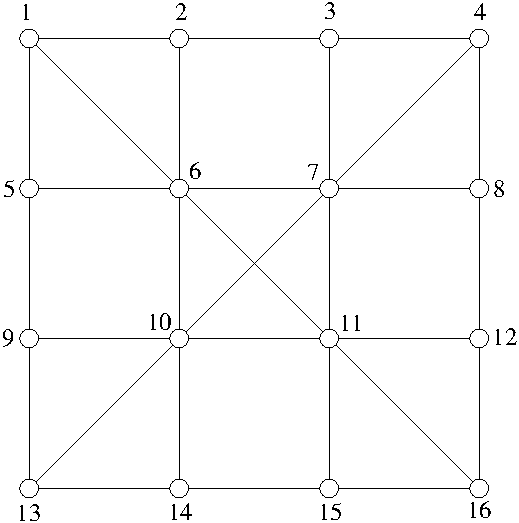
\includegraphics{../figures/mst-game}
\end{center}
\end{exercises}


\end{document}

